%%%%%%%%%%%%%%%%%%%%%%%%%%%%%%%%%%%%%%%%%
% Beamer Presentation
% LaTeX Template
% Version 1.0 (10/11/12)
%
% This template has been downloaded from:
% http://www.LaTeXTemplates.com
%
% License:
% CC BY-NC-SA 3.0 (http://creativecommons.org/licenses/by-nc-sa/3.0/)
%%%%%%%%%%%%%%%%%%%%%%%%%%%%%%%%%%%%%%%%%

%---------------------------------------------------------------
%    PACKAGES AND THEMES
%---------------------------------------------------------------
\documentclass{beamer}
\usepackage{threeparttable}
\usepackage{tikz}
\usepackage{mathrsfs}
\usepackage{ulem}
\usepackage{listings}
\usepackage{multicol}
\usepackage{bm}      % for \bm macro
\usepackage{upgreek}
\usepackage{xcolor}
\usepackage{vwcol}
\usepackage[utf8]{inputenc}
\usepackage{hhline}
\usepackage{pdfpages}
\usepackage{subcaption}
\usepackage{graphicx}
\usepackage{makecell}
\usepackage{amsmath}
\usepackage{mathtools}
\usepackage{environ}
\usepackage{fontawesome}
\usepackage{caption}
\usepackage[mode=buildnew]{standalone}
% \usepackage[backend=bibtex,style=authoryear-comp,dashed=false,natbib=true]{biblatex}
\usepackage{booktabs} % Allows the use of \toprule, \midrule and \bottomrule in tables
\usepackage{listings}
\usepackage{forloop}

\def\b{\mathbf}
\mode<presentation> {

\usetheme{Frankfurt}

%%%%% COLORS


\usecolortheme{beaver}
\definecolor{darkblue}{HTML}{00305E}
\definecolor{lowgreen}{HTML}{BCDCBC}
\definecolor{darkred}{rgb}{0.8,0,0}
\definecolor{darkgreen}{rgb}{0,0.5,0}
\definecolor{darkerred}{rgb}{0.6,0,0}
\setbeamercolor{item projected}{bg=darkblue}
\setbeamercolor{itemize item}{fg=darkblue}
\setbeamercolor{itemize subitem}{fg=darkblue}

\setbeamercolor{section number projected}{bg=darkblue}
\setbeamercolor{subsection number projected}{bg=darkblue}
\setbeamercolor{block title}{use=structure,bg=darkblue}
\setbeamercolor{block body}{use=structure,bg=darkblue!10!white}
\setbeamercolor{block title example}{use=structure,bg=lowgreen, fg=black}
\setbeamercolor{block body example}{use=structure,bg=green!3!white}
\setbeamercolor{palette primary}{bg=darkblue,fg=white}
\setbeamercolor{palette secondary}{bg=darkblue,fg=white}
\setbeamercolor{palette tertiary}{bg=darkblue!70!white,fg=white}
\setbeamercolor{palette quaternary}{bg=darkblue!60!white,fg=white}

\setbeamercolor*{title}{bg=white,fg=darkblue}
\setbeamercolor{frametitle}{fg=darkblue,bg=white}
\setbeamercolor{institute}{fg=black!70}
\setbeamercolor{date}{fg=black!70}
\usefonttheme[onlymath]{serif}
\setbeamercolor*{enumerate item}{fg=darkblue}
\setbeamercolor*{enumerate subitem}{fg=darkblue}
\setbeamercolor*{enumerate subsubitem}{fg=darkblue}
%%%% FORMATS

% \addbibresource{bibtex.bib}

% \setbeamertemplate{headline}{}
% \setbeamertemplate{footline} % Footer line
%\setbeamertemplate{footline}[page number] % Footer conter
% \setlength\bibitemsep{1.5\itemsep}
\setbeamerfont{footnote}{size=\Tiny}
\setbeamertemplate{navigation symbols}{}
\setbeamertemplate{page number in head/foot}{}
% \setbeamertemplate{bibliography item}{}
\setbeamertemplate{caption}[numbered]
\setbeamercovered{transparent}
% \renewcommand\refname{Bibliography}
\setbeamerfont{author}{size=\footnotesize}
\setbeamerfont{institute}{size=\footnotesize}
\setbeamerfont{date}{size=\footnotesize}
\graphicspath{{img/}}
\setbeamertemplate{title page}[default][colsep=-4bp,rounded=true]

\setbeamertemplate{blocks}[rounded][shadow=false]
\useinnertheme{circles}
\setbeamertemplate{section in toc}{%
\leavevmode\leftskip=5.65ex%
  \llap{\raisebox{0.2ex}{\textcolor{gray}{$\circ$}}\kern1ex}%
  \inserttocsection\par%
}

\setbeamertemplate{footline}{% 
	\hfill% 
	\usebeamercolor[fg]{page number in head/foot}% 
	\usebeamerfont{page number in head/foot}% 
  % \insertpagenumber
  \insertframenumber%
	% \,/\,\inserttotalframenumber
	\kern1.2em\vskip4.5pt% 
}

%---------------------------------------------------------
%    COMMANDS
%---------------------------------------------------------
\DeclareMathOperator*{\argmax}{argmax} 
\DeclareCaptionFormat{myformat}{\fontsize{6}{6}\selectfont#1#2#3}
\captionsetup{format=myformat}
\captionsetup[figure]{labelfont={bf},name={Figure}}
\captionsetup[table]{labelfont={bf},name={Table}}
\renewcommand{\arraystretch}{1.3}

\newcommand{\customframefont}[1]{
  \setbeamertemplate{itemize/enumerate body begin}{#1}  
	\setbeamertemplate{itemize/enumerate subbody begin}{#1}
}

\NewEnviron{framefont}[1]{
	\customframefont{#1} % for itemize/enumerate
	{#1 % For the text outside itemize/enumerate
		\BODY
	}
	\customframefont{\normalsize}
}

\newcommand\re[1]{\textcolor{darkblue}{#1}}
}
\renewcommand\cellgape{\Gape[3pt]}

\AtBeginSection[]{%
  \begin{frame}
    \begin{center}
      \LARGE \textcolor{darkblue}{\secname}
    \end{center}
  \end{frame}
}


%---------------------------------------------------------
%    CODE FORMAT
%---------------------------------------------------------

\lstset
{ %Formatting for code in appendix
    language=Prolog,
    basicstyle=\footnotesize,
    numbers=left,
    stepnumber=1,
    showstringspaces=false,
    tabsize=1,
    breaklines=true,
    breakatwhitespace=false,
    frame=single,
    xleftmargin=2em
}
%---------------------------------------------------------
%    TITLE PAGE
%---------------------------------------------------------


\title{Investigating the Utility of Answer Set Programming and Inductive Logic Techniques in Learning Two-Player Game Strategies}
\author{Susana Hahn, Atreya Shankar \\ Cognitive Systems: Language, Learning, and Reasoning (M.Sc.)}
\institute{PM - Computational Intelligence \\ Knowledge Processing and Information Systems}
\date{June 03, 2020}

\begin{document}

\begin{frame}
\titlepage % Print the title page as the first slide
\vspace{-10px}
\begin{figure}
  
\includegraphics[width=50pt]{uni-potsdam.jpg}
  \label{fig:logo}
\end{figure}
\end{frame}


%---------------------------------------------------------
%    OVERVIEW
%---------------------------------------------------------


\begin{frame}
\frametitle{Overview}
\setcounter{tocdepth}{1}
\tableofcontents 
\end{frame}


%=========================================================
\section{Introduction}
%=========================================================

\subsection{}
\begin{framefont}{\footnotesize}
  \begin{frame}
    \frametitle{Introduction}
    \begin{columns}
      \column{0.40\linewidth}
      \begin{figure}
        \centering
        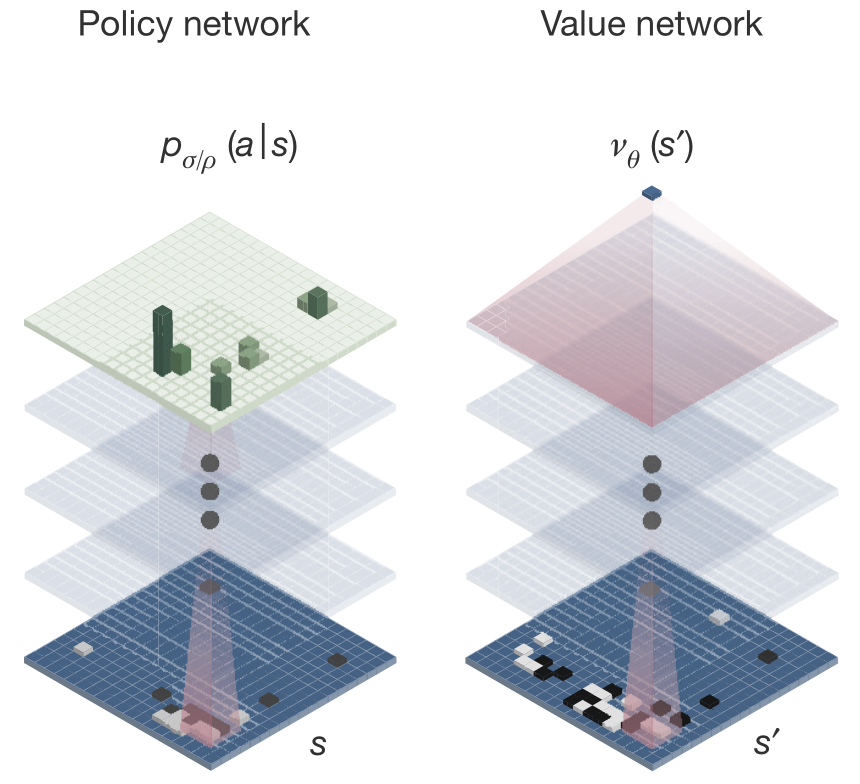
\includegraphics[trim={0.2cm -2cm 0.05cm 0.1cm},clip,width=5.3cm]{alpha_go.png}
        \captionsetup{justification=centering,margin={0.3cm,-0.8cm}}
        \caption{Schematic of policy and value neural networks in AlphaGo }
        % \citep{silver2016mastering}
      \end{figure}
      \column{0.003\linewidth}
      \column{0.60\linewidth}
      \begin{itemize}[<+->]
        \setlength\itemsep{1.2em}
        \item New advancements in computer agents using AI for two-players games \textit{AlphaGo} 
        % \citep{Silver1140}
        \begin{itemize}
          \item Deep reinforcement learning
          \item GPU hardware-acceleration 
          \item Monte-Carlo tree search
        \end{itemize}
        \item[\checkmark] Make decisions for games with exponentially complex search spaces
        \item[$\bm{\times}$] Lack of interpretability of black-box models 
        % \citep{DBLP:journals/corr/abs-1804-02477}

      \end{itemize}
    \end{columns}
  \end{frame}
\end{framefont}

\subsection{}
\begin{framefont}{\footnotesize}
  \begin{frame}
    \frametitle{Focus}
    \begin{columns}
      \column{0.40\linewidth}
      \begin{figure}
        \centering
        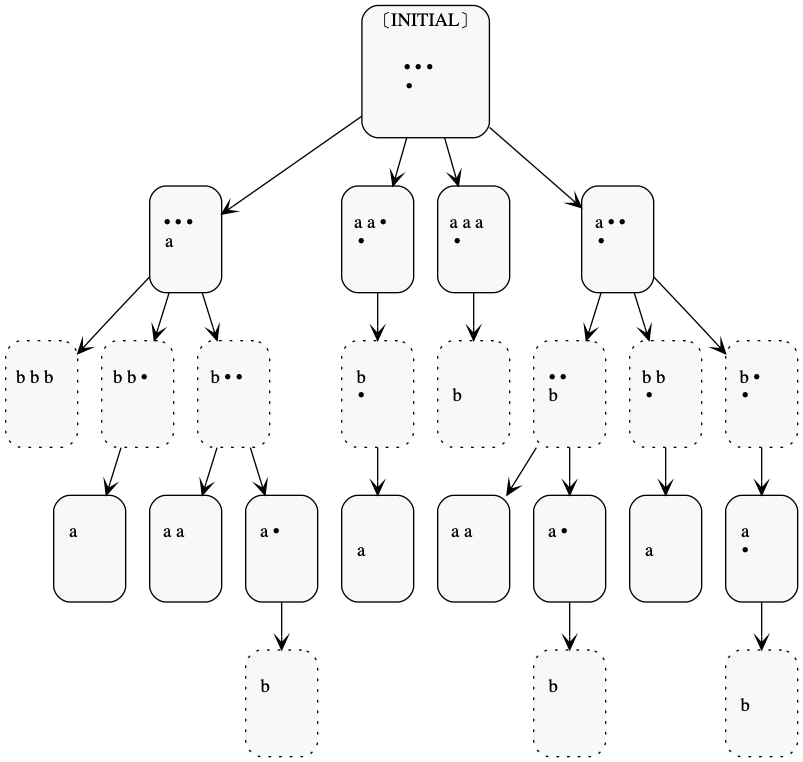
\includegraphics[trim={0cm -1cm 0cm 0cm},clip,width=5cm]{tree.png}
        \captionsetup{justification=centering,margin={0cm,-0.85cm}}
        \caption{Schematic of game tree}
        % NOTE: I think you can use this image to explain that this is a Game tree where the childs are the legal actions, since there is no section for this
      \end{figure}
      \column{0.003\linewidth}
      \column{0.60\linewidth}
      \begin{itemize}[<+->]
        \setlength\itemsep{1.2em}
      \item \re{Logic-based methods} 
      \begin{itemize}
        \item[\checkmark] Interpretability of strategies
        \item[$\bm{\times}$] Search large game spaces to learn strategies
      \end{itemize}
      \item Small two-player games: \textit{Nim} and \textit{Tic-Tac-Toe}

      \item Use formalisms from Game Description Language
      \item Use Answer Set Programming and Inductive Logic Techniques to learn \re{interpretable game-winning strategies}
      % NOTE: Note, I commented this because is misleading, there is a lot of work for multiple agents in asp, the difference here is that this is in a competitive way. So I though is better to leave it out and use something similar in the conclusion
      % \item Our method shows the potential to extend ASP from its traditional single-agent setting to that of a dynamic dual-agent setting
      \end{itemize}
    \end{columns}
  \end{frame}
\end{framefont}

\section{Background Concepts}

\subsection{}
\begin{framefont}{\footnotesize}
  \begin{frame}
    \frametitle{Two-Player Game: Nim}
    \begin{figure}
      \centering
      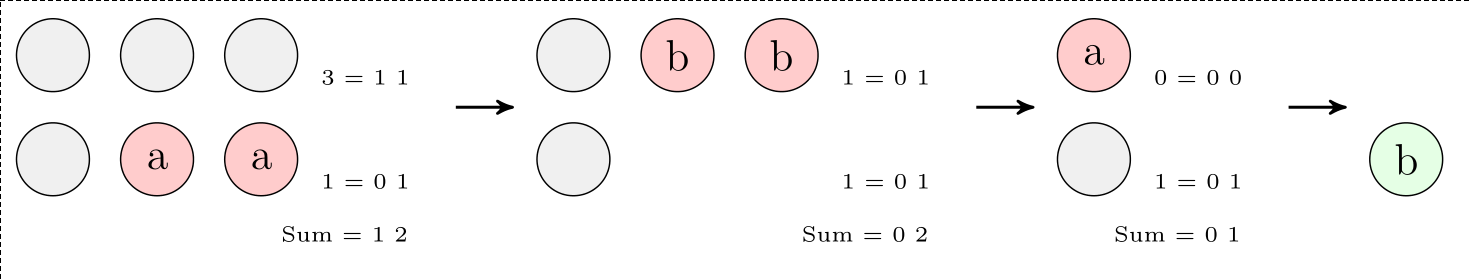
\includegraphics[trim={0.3cm -0.2cm 0.3cm 0.3cm},clip,width=10cm]{nim.png}
      \captionsetup{justification=centering,margin={0cm,0cm}}
      \caption{Schematic of Nim gameplay; red implies counters taken while green implies win}
    \end{figure}
    \begin{itemize}[<+->]
      \setlength\itemsep{0.8em}
    \item \textit{Nim} is an old game from Ancient China 
    % \citep{bouton1901nim}
    \item Players play alternately and must take at least one counter from each pile
    \item The player which takes the last counter wins the game \\ $\Longrightarrow$ there is always a winning strategy
    \item Mathematical strategy is to leave the next player with even \textit{Nim Sums}, where a \textit{Nim Sum} is the binary digital sum of counters in each pile 
    %NOTE: Discuss in which detail to explain this strategy depending on time
    \end{itemize}
  \end{frame}
\end{framefont}

\subsection{}
\begin{framefont}{\footnotesize}
  \begin{frame}
    \frametitle{Two-Player Game: Tic-Tac-Toe}
    \begin{figure}
      \centering
      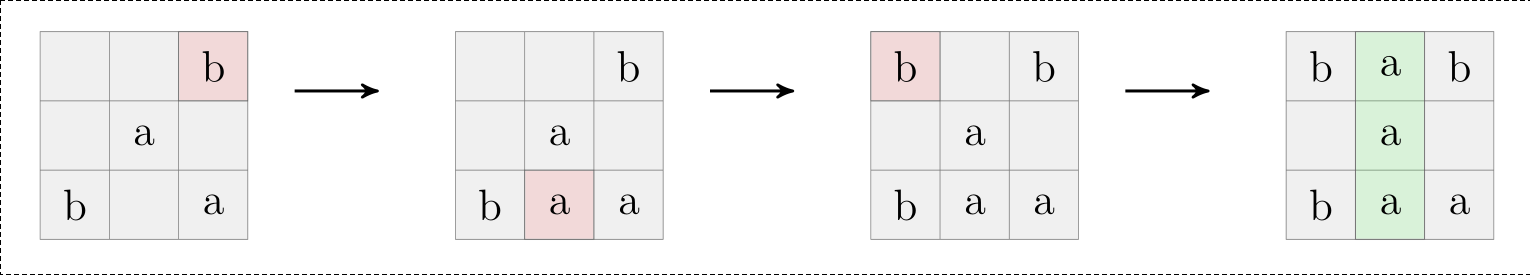
\includegraphics[trim={0.3cm 0.3cm 0.3cm 0.3cm},clip,width=10cm]{TTT.png}
      \captionsetup{justification=centering,margin={0cm,0cm}}
      \vspace{5pt}
      \caption{Schematic of Tic-Tac-Toe gameplay; red implies square taken while green implies winning streak}
    \end{figure}
    \begin{itemize}[<+->] 
      \setlength\itemsep{1em}
    \item \textit{Tic-Tac-Toe} is a $(m,n,k)$ type game which is played on a $m \times n$ size grid where each player alternately places a unique object on the grid
    \item The first player to place $k$ of its items in a row, column or diagonal wins
    \item \textit{Tic-Tac-Toe} will be treated here as a $(m,n,k)\equiv(3,3,3)$ game
    \item Unlike \textit{Nim}, a winning strategy cannot be guaranteed (might end in draw)
    \end{itemize}
  \end{frame}
\end{framefont}

\subsection{}
\begin{framefont}{\footnotesize}
  \begin{frame}
    \frametitle{Game Description Language (GDL)}
    \begin{itemize}[<+->]
      \item GDL is declarative programming language
      \item Representation formalism for axiomatising the rules of any game
    \end{itemize}
    \vspace{5pt}
    \pause
    %NOTE: I changes the title because referring to them as atoms here is strange, they are all relations even the ones with 0 attributes
    \begin{block}{Relevant GDL relations}
      $\boldsymbol{role(r)}$: $r$ is a valid role in the game \\[5pt]
      $\boldsymbol{true(p)}$: proposition $p$ is true in the current state \\[5pt]
      $\boldsymbol{next(p)}$: proposition $p$ is true in the next state \\[5pt]
      $\boldsymbol{legal(r,a)}$: player with role $r$ can legally perform action $a$ in current state \\[5pt]
      $\boldsymbol{does(r,a)}$: player with role $r$ performs action $a$ in the current state \\[5pt]
      $\boldsymbol{goal(r,n)}$: player with role $r$ achieves a utility of $n$ in the current state \\[5pt]
      $\boldsymbol{terminal}$: the current state is the final or terminal state \\[5pt]
    \end{block}
  \end{frame}
\end{framefont}

% NOTE: The ILASP part I felt it was too corwded and explaining all in detail would take too long. My idea with this reorder is that the concepts of backgroung knowledge, serach space and hypothesis can be explained while going carefully through the definition in the Overview. And then the second slide is just about the extension for weak constraints. So that it is not mixed and we strart by the basic definition of ILP then the one for ILASP using ASP and then the extension with weak constraints. We can also go back to the oder version if you find it better. 
\subsection{}
\begin{framefont}{\footnotesize}
  \begin{frame}
    \frametitle{Inductive Learning of Answer Set Programs (ILASP)}
    \begin{itemize}[<+->]
      \item \re{Inductive Logic Programming} is to find a hypothesis that explains a set of examples with some background knowledge
      \item \re{ILASP} is an inductive logic framework developed largely by Mark Law from the Imperial College London
      % \citep{law2017inductive}
    \end{itemize}
    \pause
      \begin{block}{Overview of ILASP framework}
        Given an ASP program $B$ called the \textbf{background knowledge}, a set of ASP rules $S$ called the \textbf{search space} and two sets of partial interpretations $E^{+}$ and $E^-$ called the \textbf{positive and negative examples} respectively, the goal is to find another program $H$ called a \textbf{hypothesis} such that:
        \setbeamertemplate{enumerate items}[default]
        \begin{enumerate}
        \item $H$ is composed of the rules in $S$ ($H \subseteq S$)
        \item Each positive example is extended by at least one answer set of $B \cup H$ (can be a different answer set for each positive example)
        \item No negative example is extended by any answer set of $B \cup H$
        \end{enumerate}
    \end{block}
  \end{frame}
\end{framefont}

\begin{framefont}{\footnotesize}
  \begin{frame}
    \frametitle{Inductive Learning of Answer Set Programs (ILASP)}
    \begin{itemize}[<+->]
      \item Provides a method to extend the above workflow to learn \re{weak constraints} from \re{ordered examples}
      % \citet{law2017inductive} 
      \item Particularly powerful for situations in two-player games with multiple optimum decisions with varying degrees of preference
    \end{itemize}
    \pause
    \begin{block}{Key Definitions from ILASP extension}
    \textbf{Ordering example:} An ordering example is a tuple $o = \langle e_1,e_2 \rangle$, where $e_1$ and $e_2$ are partial (positive-example) interpretations. \\[5pt]
    \textbf{Brave ordering:} An ASP program $P$ bravely respects $o$ iff $\exists A_1,A_2 \in AS(P)$, such that $AS(P)$ is the answer set of $P$, $A_1$ extends $e_1$, $A_2$ extends $e_2$ and $A_1 \succ_p A_2$.
    \end{block}
  \end{frame}
\end{framefont}

\section{Methodologies}

\subsection{}
\begin{framefont}{\footnotesize}
  \begin{frame}
    \frametitle{Overview of Methodologies}
    \begin{columns}
      \column{0.40\linewidth}
      \vspace{-20pt}
      \begin{figure}
        \centering
        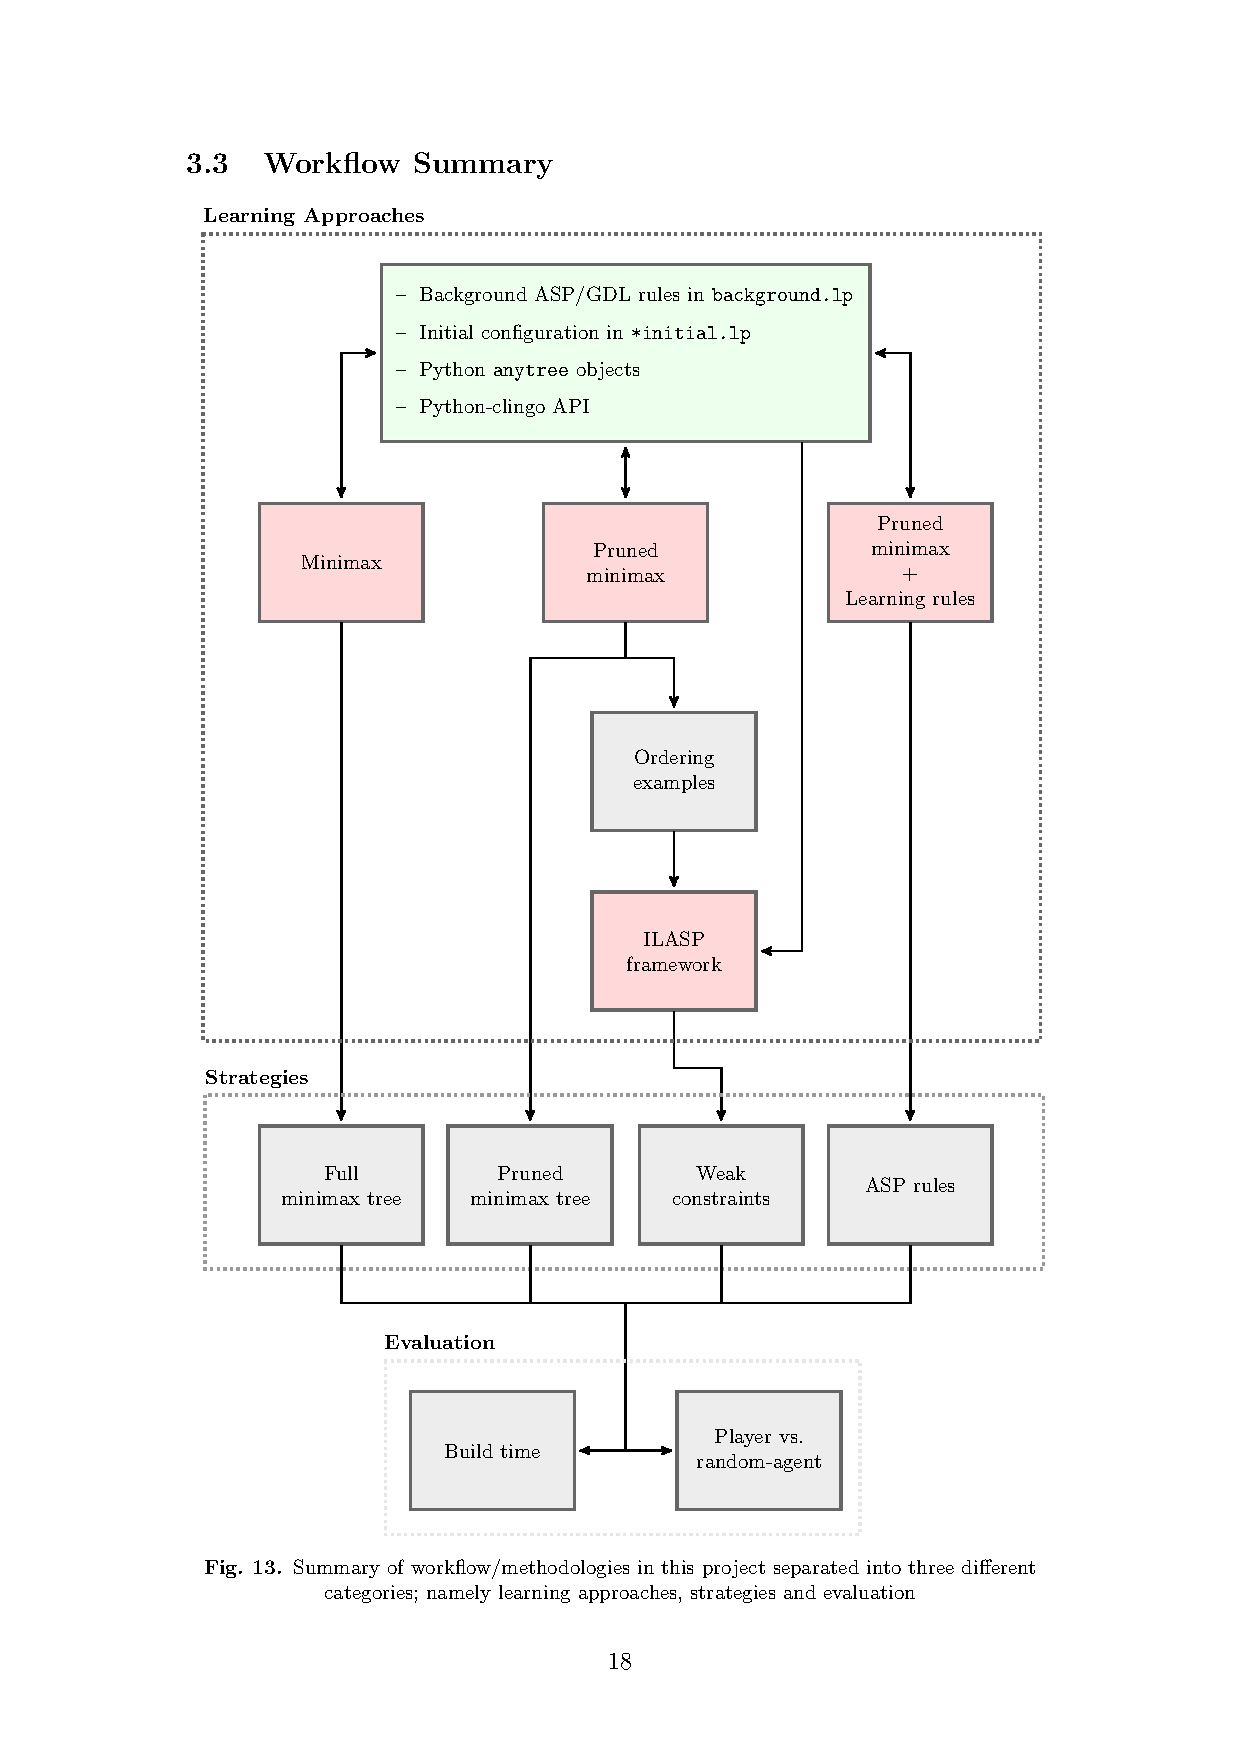
\includegraphics[trim={3cm 4cm 3cm 3.5cm},clip,width=4.8cm]{workflow.pdf}
        \captionsetup{justification=centering,margin={-0.3cm,-0.7cm}}
        \caption{Overview and segmentation of methodologies}
      \end{figure}
      \column{0.60\linewidth}
      \vspace{-20pt}
      \begin{itemize}[<+->]
        \setlength\itemsep{1.2em}
      \item Exploit ASP and python-clingo API to create a dynamic game system governed with GDL relations
      \item Python \textit{anytree} module to represent the game trees which are annotated with scores and produce pretty visualizations
      \item Flavours of the \textit{Minimax} algorithm in ASP to learn optimum game strategies
      \item Pipe optimum decisions as bravely ordered positive examples for ILASP
      \item Evaluate different methodologies by comparing build times and performance against a control (random) player
      \end{itemize}
    \end{columns}
  \end{frame}
\end{framefont}

\subsection{}
  \begin{frame}[fragile]
    \frametitle{Game simulation}
    \footnotesize
    \begin{columns}
      \begin{column}{0.48\textwidth}
        ASP program encoding the rules of the game for one step
          \begin{example}[Rules TicTacToe]
            \begin{semiverbatim}
              \footnotesize
1 \{does(X,A):legal(X,A)\} 1 :- 
  true(control(X)),
  not terminal.

next(control(a)) :- 
  true(control(b)), 
  not terminal.

goal(P,1) :- 
  true(has(P,C1)),
  true(has(P,C2)),
  true(has(P,C3)),
  in_line(C1,C2,C3).
...
      
            \end{semiverbatim}
        \end{example}
      \end{column}
      \pause
      \begin{column}{0.48\textwidth}
        Facts defining the state
        \begin{example}[State TicTacToe]
          \begin{semiverbatim}
            \footnotesize
true(control(a)).
true(free(1,3)).
true(free(3,1)).
true(free(2,3)).
...
          \end{semiverbatim}
      \end{example}
\pause
      $\big\downarrow$ (Clingo's API)
      \vspace{10px}

      One stable model per legal action
      \begin{example}[Next state TicTacToe]
        \begin{semiverbatim}
          \footnotesize
does(a,take(2,2))
next(control(b))
next(free(1,3))
next(free(2,3))
...
        \end{semiverbatim}
    \end{example}
      \end{column}
  \end{columns}

\end{frame}



\subsection{}
\begin{framefont}{\footnotesize}
  \begin{frame}
    \frametitle{Minimax Algorithm}
    \begin{figure}
      \centering
      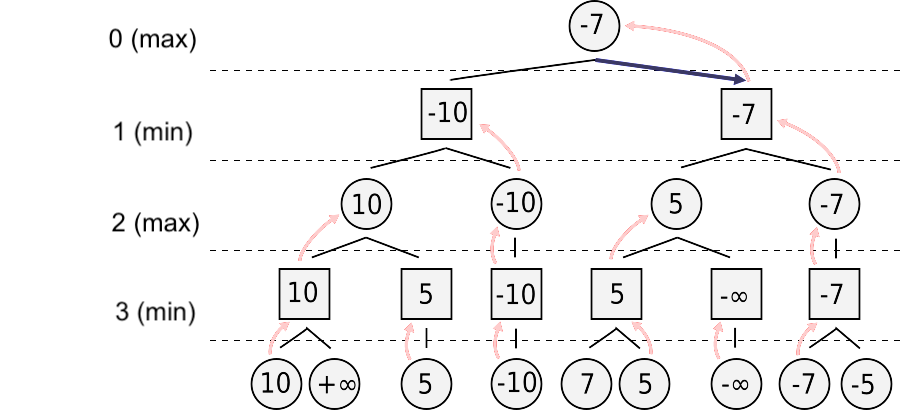
\includegraphics[trim={0cm -0.5cm 0cm 0cm},clip,width=9cm]{Minimax.png}
      \captionsetup{justification=centering,margin={0cm,0cm}}
      \caption{Minimax sample schematic for a two-player game }
      % \citep{wiki:xxx}
    \end{figure}
    \vspace{-10pt}
    \begin{itemize}[<+->]
    \item One player maximizes utility while another minimizes utility
    \item Bottom-Up procedure assuming there is a complete game tree with utility-annotated leaf nodes
    \item Time complexity: $O(b^D)$; Space complexity: $O(bD)$; where $b$ is the average branching factor and $D$ is the maximum depth of the tree 
    % \citep{russell2016artificial}
    \end{itemize}
  \end{frame}
\end{framefont}

\subsection{}
\begin{framefont}{\footnotesize}
  \begin{frame}
    \frametitle{Minimax Algorithm}
    \begin{figure}
      \centering
      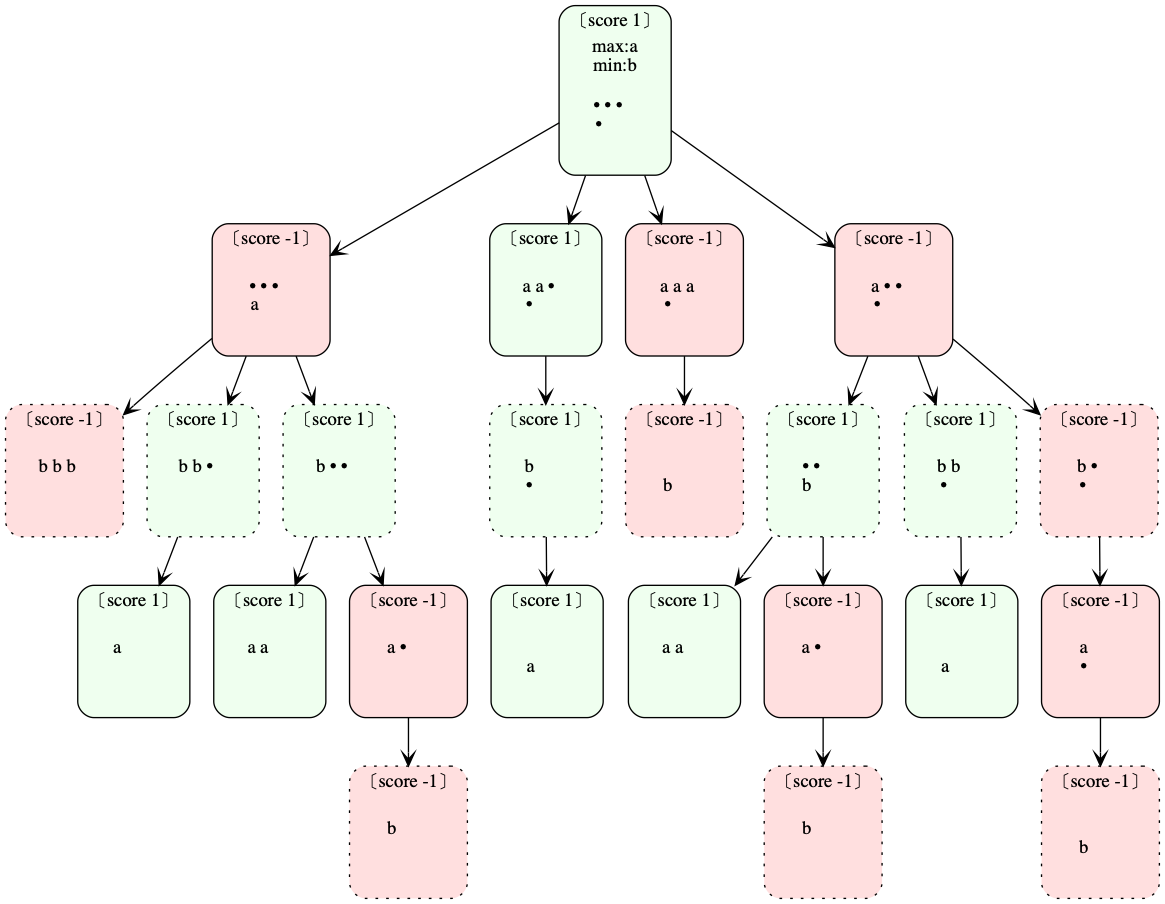
\includegraphics[trim={0cm -0.5cm 0cm 0cm},clip,width=8.5cm]{tree-minmax.png}
      \captionsetup{justification=centering,margin={0cm,0cm}}
      \caption{Minimax schematic for a small Nim game where player $a$ maximizes utility while player $b$ minimizes utility; using the Minimax algorithm we can deduce that player $a$ starts off with a winning strategy}
    \end{figure}
  \end{frame}
\end{framefont}


\subsection{}
\begin{framefont}{\footnotesize}
  \begin{frame}
    \frametitle{Pruned Minimax Algorithm}
    \re{Motivation}
    \begin{itemize}[<+->]
      \item Construct only the necessary parts of the tree (Alphabeta pruning)
      \item Treat it as a planning problem
      \item Use optimization statements from \textit{clingo}
    \end{itemize}

    \pause
    Explicit time encoding
    \setbeamertemplate{enumerate items}[default]
    \begin{enumerate}[<+->]
      \item Replace \texttt{true(F)} by \texttt{holds(F,T)}
      \item Replace \texttt{next(F)} by \texttt{holds(F,T+1)}
      \item Replace \texttt{p(F1..Fn)} by \texttt{p(F1..Fn,T)} for $\{ legal,does,goal,terminal\}$
      \item Add the time in in the body with predicate \texttt{time(T)}
      \item Add a new fact \texttt{time(0..N).} for horizon $N$
      \end{enumerate}
      \pause
      Optimization statements
      \begin{itemize}[<+->]
        \item \texttt{\#maximize\{N,T:goal(a,N,T)\}}
        \item[$\times$] Assumes player $b$ will chose actions under the same optimization. 
      \end{itemize}
  \end{frame}
\end{framefont}

\subsection{}
\begin{framefont}{\footnotesize}
  \begin{frame}
    \frametitle{Pruned Minimax Algorithm}
    
    
    \includegraphics<1>[width=0.9\textwidth,height=0.9\textheight,keepaspectratio]{tree-pruned-1.png}
    \includegraphics<2>[width=0.9\textwidth,height=0.9\textheight,keepaspectratio]{tree-pruned-2.png}
    \includegraphics<3>[width=0.9\textwidth,height=0.9\textheight,keepaspectratio]{tree-pruned-3.png}
    \includegraphics<4>[width=0.9\textwidth,height=0.9\textheight,keepaspectratio]{tree-pruned-4.png}
    \includegraphics<5>[width=0.9\textwidth,height=0.9\textheight,keepaspectratio]{tree-pruned-5.png}
    \includegraphics<6>[width=0.9\textwidth,height=0.9\textheight,keepaspectratio]{tree-pruned-6.png}
    \includegraphics<7>[width=0.9\textwidth,height=0.9\textheight,keepaspectratio]{tree-pruned-7.png}
    \includegraphics<8>[width=0.9\textwidth,height=0.9\textheight,keepaspectratio]{tree-pruned-8.png}
    \includegraphics<9>[width=0.9\textwidth,height=0.9\textheight,keepaspectratio]{tree-pruned-9.png}
    \includegraphics<10>[width=0.9\textwidth,height=0.9\textheight,keepaspectratio]{tree-pruned-10.png}

  \end{frame}
\end{framefont}

  \begin{frame}[fragile]
    \frametitle{Pruned Minimax Algorithm}
    \footnotesize
    \setbeamertemplate{enumerate items}[default]
      \re{Learn Rules:} Create a representation of the best moves using ASP
      \pause
    \begin{example}
      \begin{semiverbatim}
best\_do(a,remove(2,2),T):- holds(control(a),T), holds(has(1,0),T), 
                          holds(has(2,2),T), holds(has(3,0),T), 
                          holds(has(4,0),T).
      \end{semiverbatim}
    \end{example}
    \pause
    Enforce the use of these best actions
    \begin{semiverbatim}
1\{does(P,A,T):best\_do(P,A,T)\}1:- time(T), not goal(\_,\_,T),
                                {best\_do(P,A,T)}>0, true(control(P)).
    \end{semiverbatim}
    \pause
    Generalize using predefined options for substitution 
    \begin{example}
      \begin{semiverbatim}
best_do(Va,remove(V2,1),T):- holds(control(Va),T), 
                        holds(has(V1,0),T), holds(has(V2,2),T),
                        holds(has(V3,0),T), holds(has(V4,0),T), 
                        V1!=V3,V1!=V2,V1!=Va, 
                        V3!=V2,V3!=Va,V2!=Va.
      \end{semiverbatim}
    \end{example}
\end{frame}

% \begin{framefont}{\footnotesize}
%   \begin{frame}
%     \frametitle{Pruned Minimax Algorithm}
%     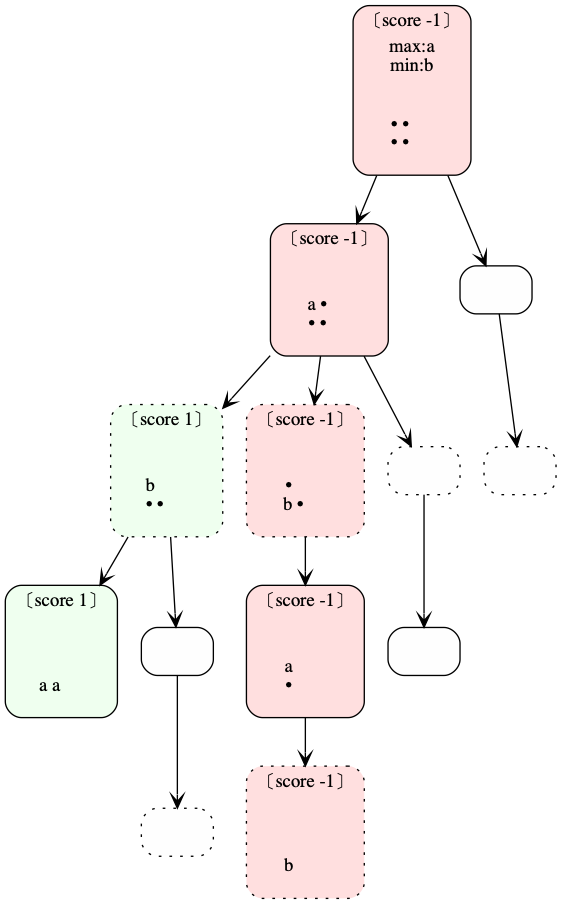
\includegraphics[width=0.9\textwidth,height=0.9\textheight,keepaspectratio]{tree-rules.png} 
%   \end{frame}
% \end{framefont}

\subsection{}
\begin{frame}[fragile]
  \frametitle{Weak constraints with ILASP}
  \footnotesize
  \begin{itemize}[<+->]
    \item \re{Background Knowledge}: Encoding with rules\\
    \item \re{Ordered positive examples}: Generated in the decision points of Pruned Minimax
  \end{itemize}
  \pause
  \begin{example}
    \begin{semiverbatim}
#pos(e0,\{\}, \{\},\{ 
  true(control(a)). true(has(1,0)). true(has(2,2)). 
  true(has(3,0)). true(has(3,0)). does(a,remove(2,2)).\}).
#pos(e1,\{\}, \{\}, \{
  true(control(a)). true(has(1,0)). true(has(2,2)).
  true(has(3,0)). true(has(4,0)). does(a,remove(2,1)). \}).      
#brave_ordering(e0,e1).    
  \end{semiverbatim}
  \end{example}
  \pause
  \begin{itemize}[<+->]
    \item \re{Language bias}: Must be handcrafted to define the search space of the ILASP framework\\
    \item[$\Longrightarrow$] \re{Hypotheses}: Weak constraints representing the strategy
  \end{itemize}
\end{frame}

\begin{frame}[fragile]
  \footnotesize
  
  
  \begin{example}[Language bias TicTacToe]
    \begin{semiverbatim}
#modeo(3,next(has(var(player),var(cell))),(positive)).
#modeo(1,in\_line(var(cell),var(cell),var(cell)),(positive)).
#modeo(1,next(free(var(cell))),(positive)).
#modeo(1,next(control(var(player))),(positive)).
#weight(-1). #weight(1).
#maxp(2). #maxv(4). 
  \end{semiverbatim}
  \end{example}
  \pause
  \begin{example}[Language bias Nim]
    \begin{semiverbatim}
#constant(pile,1..4). 
#modeh(b(var(pile),var(d),var(bool)),(positive)).
#modeh(nim\_sum(var(d),var(total)+var(bool),var(pile)),(positive)).
#modeh(nim_sum(var(d),0,0),(positive)).
#modeb(1,b(var(pile),var(d),var(bool)),(positive)).
#modeb(1,nim\_sum(var(d),var(total),var(pile)-1),(positive)).
#modeb(1,binary(var(num),var(d),var(bool)),(positive)).
#modeb(1,next(has(var(pile),var(num))),(positive)).
#modeo(1,nim\_sum(var(d),var(t),const(pile))).
#modeo(1,var(t)\\2 != 0).
#weight(1). #weight(-1).
#maxp(1). #maxv(4).
  \end{semiverbatim}
  \end{example}

\end{frame}

%=========================================================
\section{Results}
%=========================================================

\subsection{}
\begin{framefont}{\footnotesize}
  \begin{frame}
    \frametitle{Setup}
    \begin{itemize}[<+->]
      \item Time to learn strategy and its size
      \item Abstraction of strategy from a smaller instance
      \item 2.6 GHz Quad- Core Intel Core i7 processor under MacOs
    \end{itemize}
    \includegraphics<4>[width=0.9\textwidth,height=0.9\textheight,keepaspectratio]{test-instances.png}
  \end{frame}
\end{framefont}

\subsection{}
\begin{framefont}{\footnotesize}
  \begin{frame}
    \frametitle{Learning phase}
\begin{table}[]
    \begin{tabular}{*7l}
    \toprule
\textbf{Approach} &  \multicolumn{3}{c}{\textit{Nim}} & \multicolumn{3}{c}{\textit{TicTacToe}}\\
  \midrule
  
  {} & S  & M & L & S  & M & L
  \\
  \midrule[0.35mm]
  \textbf{Minimax}  & 390 & 4630 & 61023
  & 896 & 7583 & 59704
  \\[20pt]
  \textbf{Pruned minimax tree}   & 83 & 347 & 2675 & 105 & 73 & 2835
  \\[20pt]
  \textbf{Pruned minimax rules} & 35 & 85 & 283 & 109 & 61 & 2399 
  \\
\bottomrule
\end{tabular}
\caption{Number of nodes in the computed trees}

\end{table}
    
  \end{frame}
\end{framefont}


\begin{frame}[fragile]
  \footnotesize
  \frametitle{Learning phase ILASP strategies}


  \begin{example}[Nim instances \textit{M} and \textit{L}]
    \begin{semiverbatim}
nim\_sum(V1,0,0) :- b(\_,V1,\_).
nim\_sum(V1,V3+V2,V0) :- b(V0,V1,V2), nim\_sum(V1,V3,V0-1).
b(V3,V1,V2) :- binary(V0,V1,V2), next(has(V3,V0)).
:~ nim\_sum(V0,V1,4), V1\\2 != 0.[1@1, 4, V0, V1]
  \end{semiverbatim}
  \end{example}
  \pause
  \begin{example}[TicTacToe instance \textit{S}]
    \begin{semiverbatim}
:~ next(has(V0,V1)), in_line(V1,V2,V3).[1@1, 1, V0, V1, V2, V3]
:~ in_line(V0,V1,V2), next(free(V0)).[-1@2, 2, V0, V1, V2]
:~ next(has(V0,V1)), in_line(V2,V3,V1), 
    next(free(V2)).[1@2, 3, V0, V1, V2, V3]
:~ next(has(V0,V1)), next(has(V0,V2)), 
    next(has(V0,V3)), in_line(V1,V2,V3).[-1@2, 4, V0, V1, V2, V3]
  \end{semiverbatim}
  \end{example}

\end{frame}


\begin{framefont}{\footnotesize}
  \begin{frame}
    \frametitle{Learning phase}
    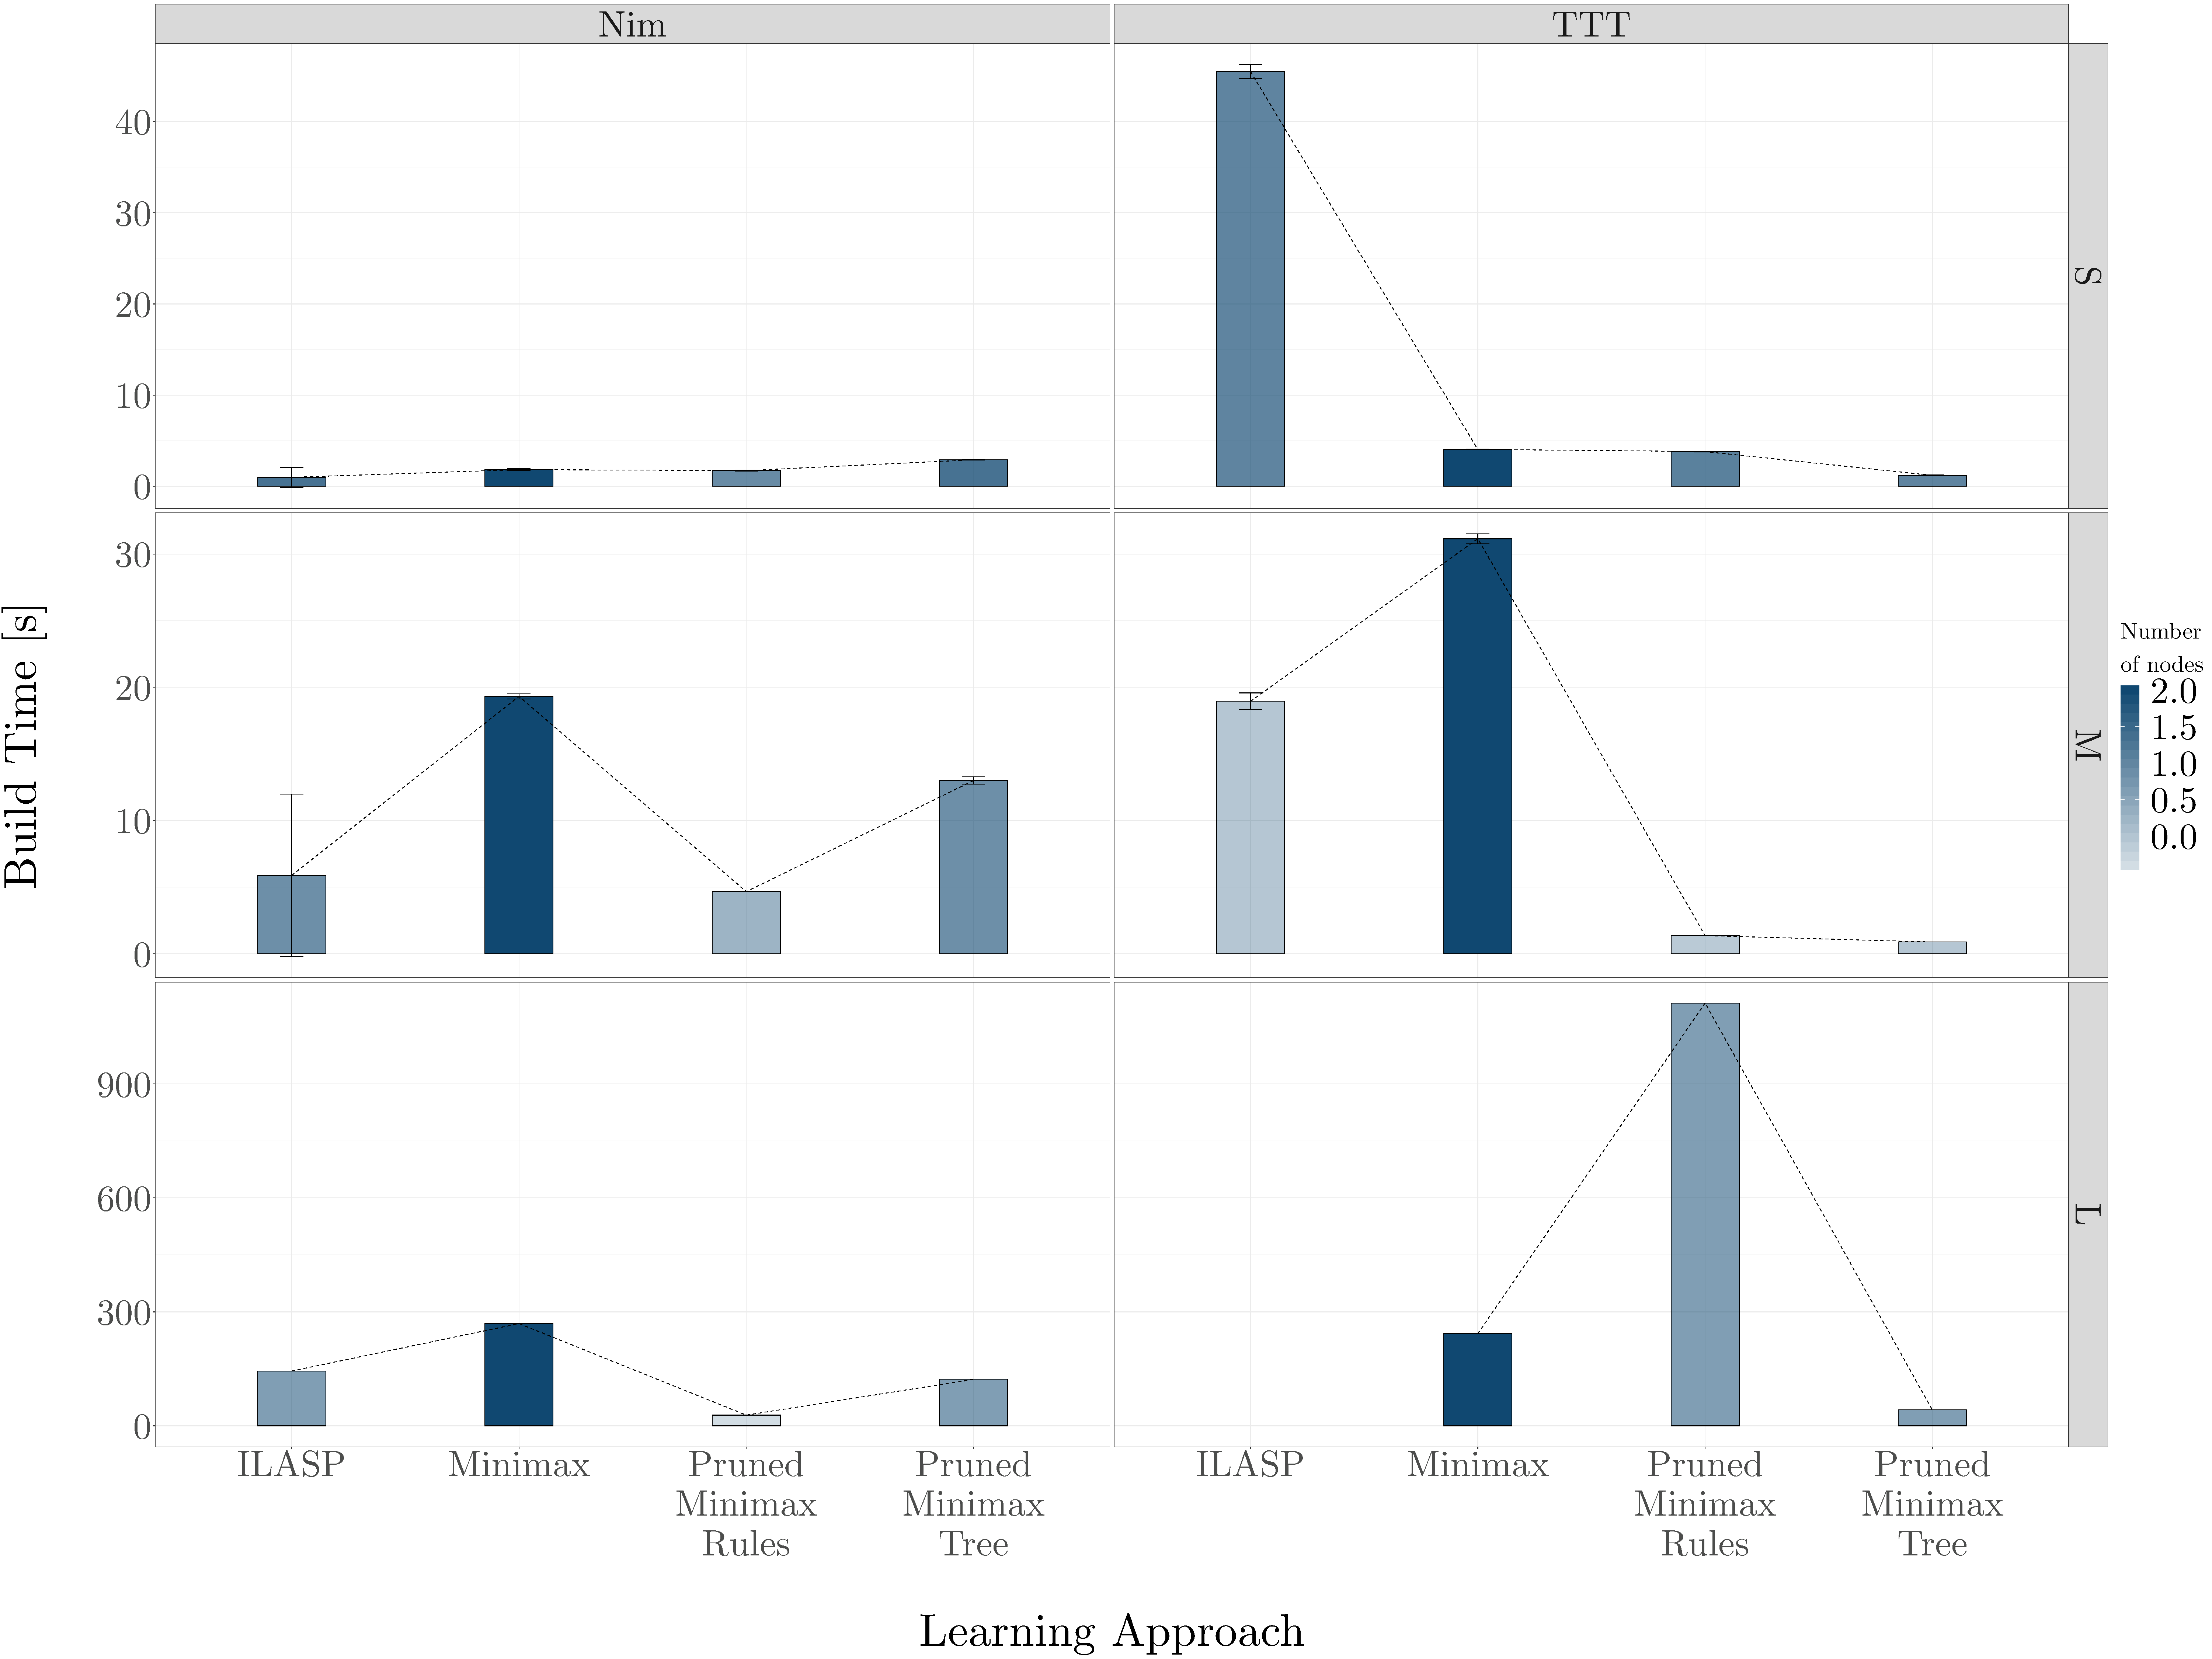
\includegraphics[width=\textwidth,height=0.9\textheight,keepaspectratio]{bar_build.pdf}
  \end{frame}
\end{framefont}


\begin{framefont}{\footnotesize}
  \begin{frame}
    \frametitle{Play against Random-Agent}
    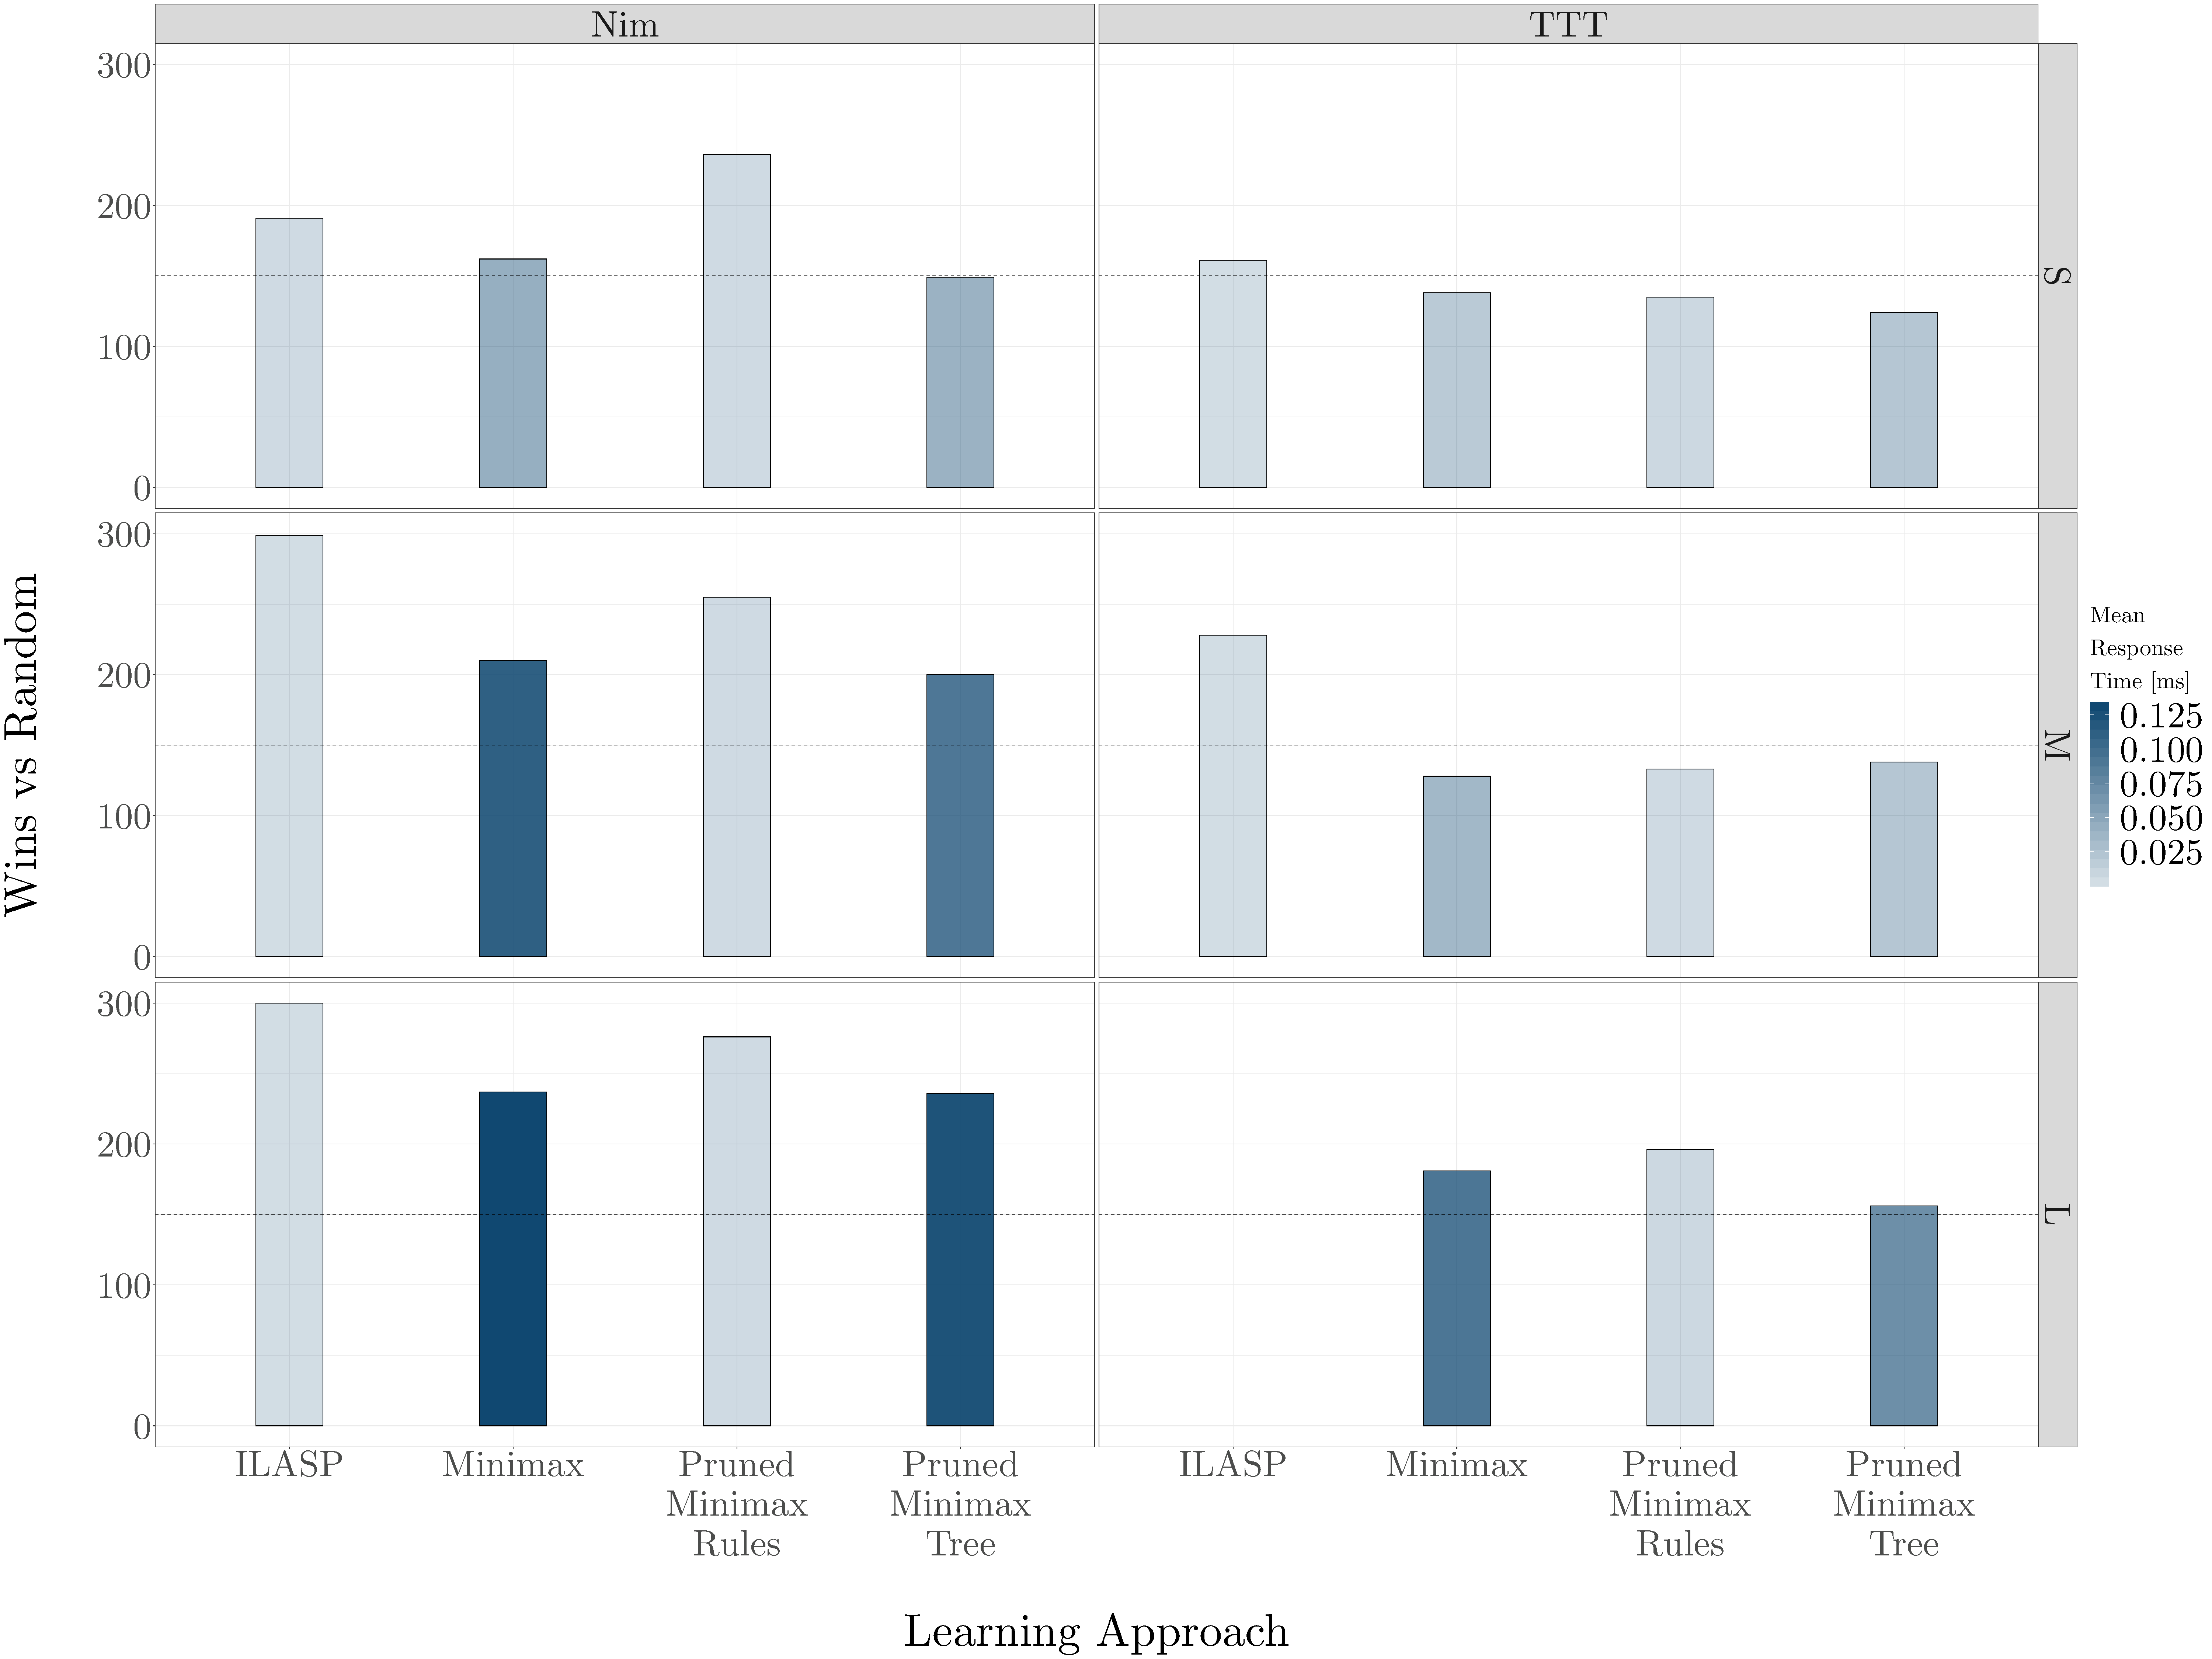
\includegraphics[width=\textwidth,height=0.9\textheight,keepaspectratio]{bar_vs.pdf}
  \end{frame}
\end{framefont}


%=========================================================
\section{Conclusion}
%=========================================================

\subsection{}
\begin{framefont}{\footnotesize}
  \begin{frame}
    \frametitle{Conclusion}
    \begin{multicols}{2}
    \begin{itemize}[<+->]
      \item Minimax
      \begin{itemize}
        \item[\checkmark] Good for small instances
        \item[$\times$] Slow learning and not scalable
      \end{itemize}
      \item Pruned Minimax
      \begin{itemize}
        \item[\checkmark] Reduces tree search space
        \item[\checkmark] Allow generalization based on symmetries
        \item[\checkmark] Novel approach
      \end{itemize}
      \item ILASP
      \begin{itemize}
        \item[\checkmark] Explainable abstract strategies
        \item[$\times$] Dependent on language bias
      \end{itemize}
    \end{itemize}
    \columnbreak
    \pause
    \re{Our framework}
    \pause
    \begin{itemize}[<+->]
      \item Using ASP for the game dynamics
      \item Extendible with new learning approaches
      \item Customizable games
      \item Command line tools
      \item Game Tree visualizations
    \end{itemize}
  \end{multicols}
    

  \end{frame}
\end{framefont}
%=========================================================
\section{Bibliography}
%=========================================================
\begin{frame}[plain]
  \nocite{*} 
  \setbeamertemplate{bibliography item}{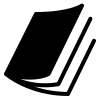
\includegraphics[width=1em]{./bibicon.png}}
  \frametitle{References}
  \bibliographystyle{plainnat}
  \begin{multicols}{2}
    \tiny\bibliography{./bibtex}
  \end{multicols}
\end{frame}

% \begin{frame}[allowframebreaks]
% 	\frametitle{Bibliography}
% 	\nocite{*}
% 	\printbibliography[title = {Bibliography}]
%   % \setbeamertemplate{bibliography item}{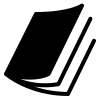
\includegraphics[width=1em]{./bibicon.png}}
% \end{frame}

\end{document}
